\documentclass{standalone}
\usepackage{tikz}
\usetikzlibrary{shapes.geometric}
\begin{document}
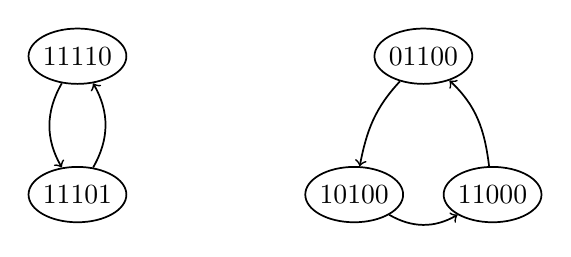
\begin{tikzpicture}
[every node/.style={inner sep=0pt}]
\node (1) [ellipse, minimum size=20.0pt, fill=white, line width=0.625pt, draw=black] at (37.5pt, -25.0pt) {\textcolor{black}{11110}};
\node (2) [ellipse, minimum size=20.0pt, fill=white, line width=0.625pt, draw=black] at (37.5pt, -75.0pt) {\textcolor{black}{11101}};
\node (3) [ellipse, minimum size=20.0pt, fill=white, line width=0.625pt, draw=black] at (162.5pt, -25.0pt) {\textcolor{black}{01100}};
\node (4) [ellipse, minimum size=20.0pt, fill=white, line width=0.625pt, draw=black] at (137.5pt, -75.0pt) {\textcolor{black}{10100}};
\node (5) [ellipse, minimum size=20.0pt, fill=white, line width=0.625pt, draw=black] at (187.5pt, -75.0pt) {\textcolor{black}{11000}};
\draw [line width=0.625, ->, color=black] (1) to  [in=120, out=240] (2);
\draw [line width=0.625, ->, color=black] (2) to  [in=300, out=60] (1);
\draw [line width=0.625, ->, color=black] (3) to  [in=79, out=227] (4);
\draw [line width=0.625, ->, color=black] (4) to  [in=210, out=330] (5);
\draw [line width=0.625, ->, color=black] (5) to  [in=317, out=97] (3);
\end{tikzpicture}

\end{document}
